\chapter{Independently Controllable Factors}

\section{Additional details}
\subsection{Architecture}
Our architecture is as follows: the encoder, mapping the raw pixel state to a latent representation, is a 4-layer convolutional neural network with batch normalization \citep{ioffe2015batch} and leaky ReLU activations. The decoder uses the transposed architecture with ReLU activations. The noise $z$ is sampled from a 2-dimensional gaussian distribution and both the generator $\Phi(h,z)$ and the policy $\pi(h,\phi)$ are neural networks consisting of 2 fully-connected layers. In practice, a minibatch of $n = 256$ or $1024$ vectors $\phi_1, \dots, \phi_{n}$ is sampled at each step. The agent randomly choses one $\phi = \phi_{behavior}$ and samples actions from its policy $a \sim \pi(h, \phi_{behavior})$. Our model parameters are then updated using policy gradient with the REINFORCE estimator and a state-dependent baseline and importance sampling. For each selectivity reward, the term $\mathbb{E}_{\phi'}[  A(h', h,\phi')]$ is estimated as $\tfrac{1}{n} \sum_{i = 1}^n A(h', h,\phi_i)$.

In practice, we don't use concatenation of vectors when feeding two vectors as input for a network (like $(h, z)$ for the factor generator or $(h, \phi)$ for the policy).
For vectors $a,b \in \mathbb{R}^{n_a \times n_b}$. We use a bilinear operation $bil(a, b) = (a_i * b_j)_{i \in [[n_a]], j \in [[n_b]]}$ as in \cite{florensa2017stochastic}.  We observe the bilinear integrated input to more strongly enforce dependence on both vectors; in contrast, our models often ignored one input when using a simple concatenation.

Through our research, we experiment with different outputs for our generator $\Phi(h,z)$.  We explored embedding the $\phi$-vectors into a hypercube, a hypersphere, a simplex and also a simplex multiplied by the output of a $tanh(\cdot)$ operation on a scalar.

\subsection{First experiment}
In the first experiment, figure~\ref{fig:dis_space}, we used a gaussian similarity kernel i.e $A(h', h, \phi) = \exp(- \frac{||h' - (h+\phi)||^2}{2 \sigma^2})$ with $\sigma = \sqrt{dim(h)}$.
In this experiment only, for clarity of the figure, we only allowed permissible actions in the environment (no no-op action).


% Our attribute selector $A(dh, \phi)$ is a gaussian kernel.

\section{Additional Figures}
\subsection{Discrete simple case}
\label{sec:sel-only}
Here we consider the case where we learn a latent space $H$ of size $K$, with $K$ factors corresponding to the coordinates of $h$ ($h_i,\; i\in[k])$, and learn $K$ separately parameterized policies $\pi_i(a|h),\;i\in[k]$. We train our model with the selectivity objective, but no autoencoder loss, and find that we correctly recover independently controllable features on a simple environment.
{%We also find experimentally that training discrete independently controllable features without training the autoencoder objective correctly recovers ground truth features and their associated control policies. 
Albeit slower than when jointly training an autoencoder, this shows that the objective we propose is strong enough to provide a learning signal for discovering a disentangled latent representation.
}

{We train such a model on a gridworld MNIST environment, where there are two MNIST digits \nocite{lecun1998mnist}. The two digits can be moved on the grid via 4 directional actions (so there are 8 actions total), the first digit is always odd and the second digit always even, so they are distiguishable. In Figure \ref{fig:gridworld-only-sel} we plot each latent feature $h_k$ as a curve, as a function of each ground truth. For example we see that the black feature recovers $+x_1$, the horizontal position of the first digit, or that the purple feature recovers $-y_2$, the vertical position of the second digit.}
\begin{figure}[H]
\centering
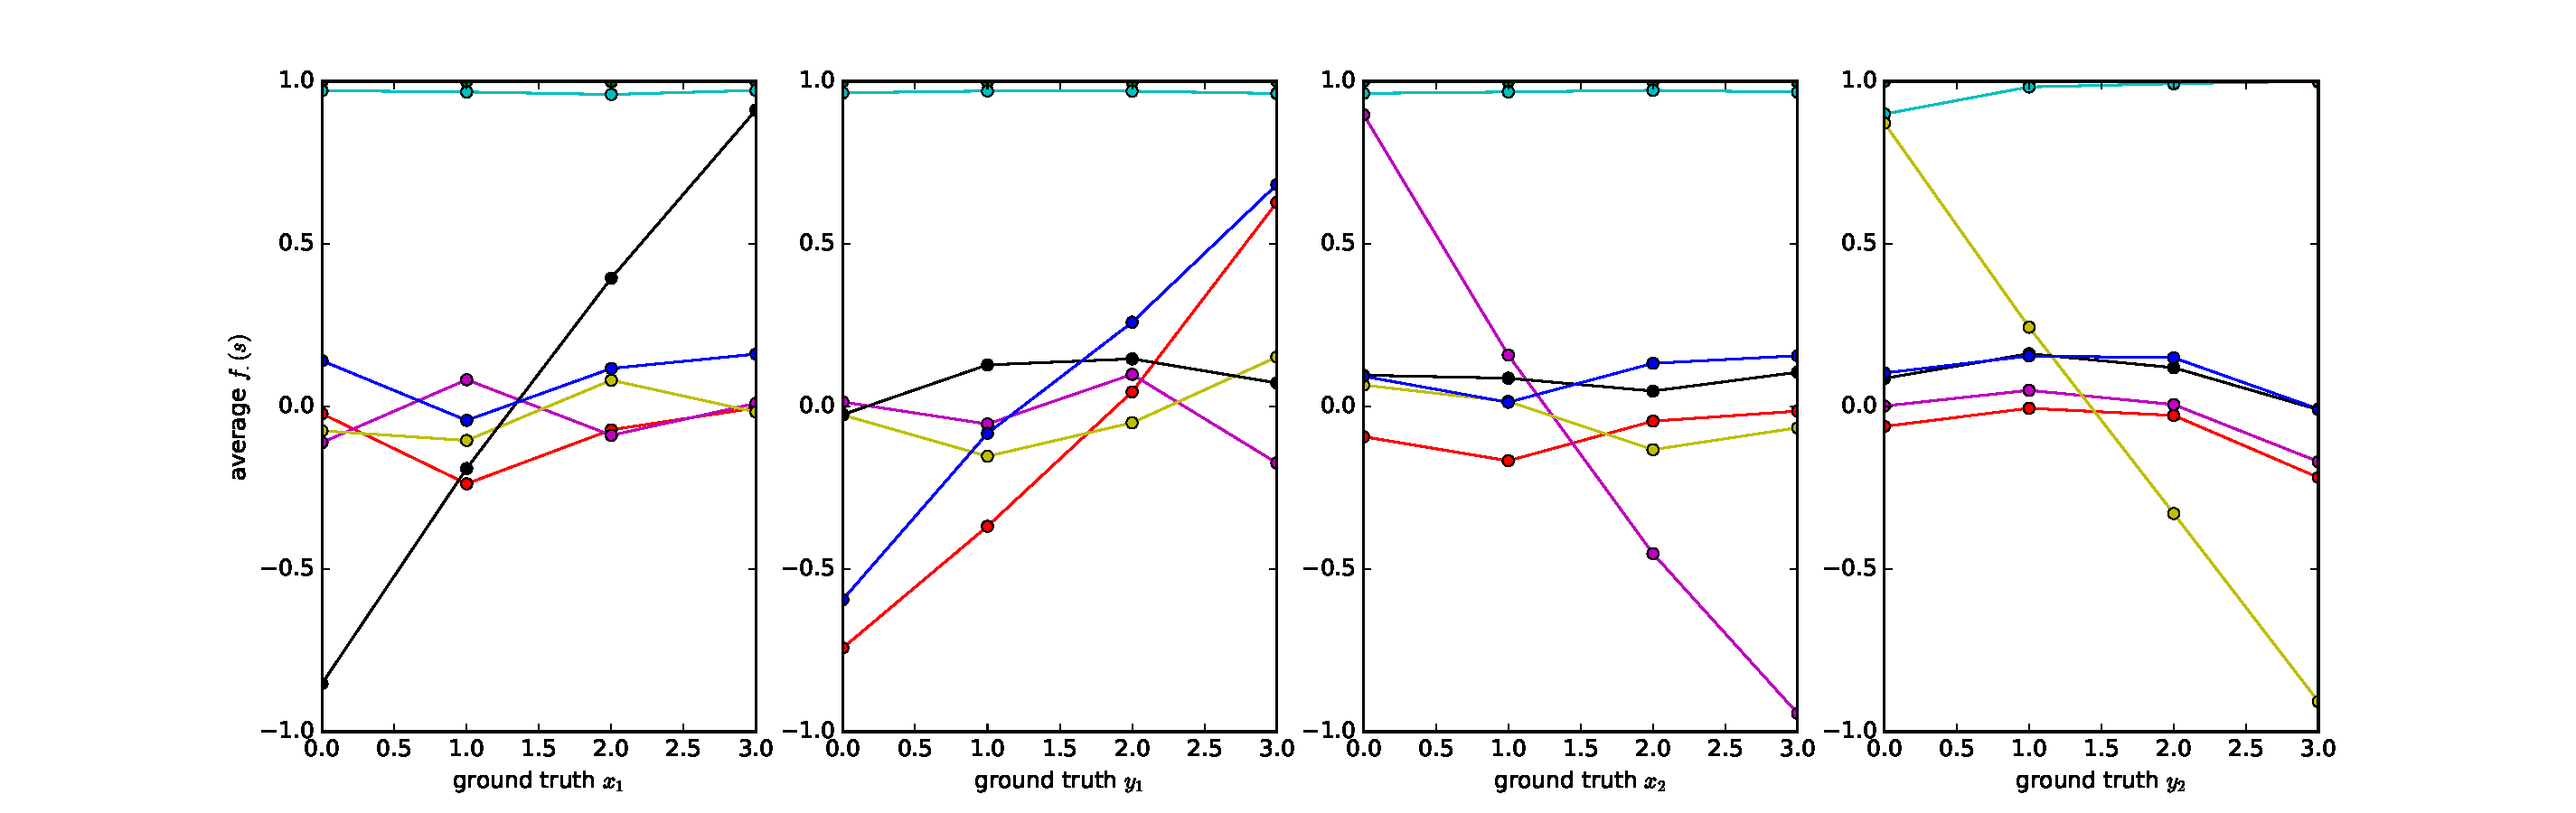
\includegraphics[width=\linewidth]{articles/icf/figures/latent_vs_gt_005.pdf}
\caption{{%Each curve represents a latent feature $f_k$ as a function of some ground truth. Here there are 4 ground truths, the $x$ and $y$ position of each of the 2 MNIST digits.
In a gridworld environment with 2 objects (in this case 2 MNIST digits), we know there are 4 underlying features, the $(x_i,y_i)$ position of each digit $i$. Here each of the four plots represents the evolution of the $f_k$'s as a function of their underlying feature, from left to right $x_1$, $y_1$, $x_2$, $y_2$. We see that for each of them, at least one $f_k$ recovers it almost linearly, from the raw pixels only.}
}
\label{fig:gridworld-only-sel}
\end{figure}


\subsection{Planning and policy inference example in 1-step}
\label{sec:exp-mb-ppi}

This disentangled structure could be used to address many challenging issues in reinforcement learning. We give two examples in figure~\ref{fig:prediction_recovering}: 
\begin{itemize}
\item Model-based predictions: Given an initial state, $s_0$, and an action sequence $a_{\{0:T-1\}}$, %the agent performed, our goal is to predict the resulting state $s_T$.
we want to predict the resulting state $s_T$.

\item A simplified deterministic policy inference problem: Given an initial state $s_{start}$ and a terminal state $s_{goal}$, we aim to find a suitable action sequence $a_{\{0:T-1\}}$ such that $s_{goal}$ can be reached from $s_{start}$ by following it.
\end{itemize}
Because of the $tanh$ activation on the last layer of $\Phi(h, z)$, the different factors of variation $dh = h' - h$ are placed on the vertices of a hypercube of dimension $K$, and we can think of the the policy inference problem as finding a path in that simpler space, where the starting point is $h_{start}$ and the goal is $h_{goal}$. We believe this could prove to be a much easier problem to solve.

\begin{figure}[H]
\centering
\subfloat[]{\scalebox{.6}{
\begin{tikzpicture}
\node[inner sep=0pt] (im0) at (0,0)
    {\fbox{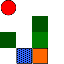
\includegraphics[width=.25\textwidth]{articles/icf/figures/im0_good.png}}};
\node[inner sep=0pt] (im1) at (5,0)
    {\fbox{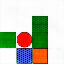
\includegraphics[width=.25\textwidth]{articles/icf/figures/im1_good.png}}};


\node[] (ht) at (0,-4) {$\underbrace{h}_{(0.4,\ 13.1)}$};
\node[] (ht1) at (7,-4) {$\underbrace{\hat{h'}}_{(-4.6,\ -1.9)} = h + \underbrace{dh_{{\color{right} {\color{right} right}}}}_{(5,\ -5)} + \underbrace{2\cdot dh_{{\color{down} down}}}_{(-10,\ -10)}$}; 
    \draw[->,thick] (im0.south) -- (ht.north)
    node[midway,fill=white] {Encoder};
    \draw[->,thick] (5, -3.3) -- (im1.south)
    node[midway,fill=white] {Decoder};
    
    \draw[->,thick] (ht.east) -- (ht1.west);
    
\end{tikzpicture}}}
\hfill
%\subfloat[]{\includegraphics[width=.3\linewidth]{./images/pdoth_tsne_p.png}}
\subfloat[]{\scalebox{.6}{
\begin{tikzpicture}
\node[inner sep=0pt] (im0) at (0,0)
    {\fbox{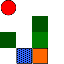
\includegraphics[width=.25\textwidth]{articles/icf/figures/im_causal0_good.png}}};
\node[inner sep=0pt] (im1) at (5,0)
    {\fbox{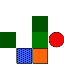
\includegraphics[width=.25\textwidth]{articles/icf/figures/im_causal1_good.png}}};


\node[] (ht) at (0,-3.5) {$\underbrace{h_1}_{(0.4,\ 13.1)}$};
\node[] (ht1) at (5,-3.5) {$\underbrace{h_2}_{(5.9,\ -11.6)}$}; 
\node[] (dh) at (2.5,-5) {$dh ={(5.5,\ -24.8)} \approx 2\cdot dh_{{\color{down} down}} + 3\cdot dh_{{\color{right} right}}$};
    \draw[->,thick] (im0.south) -- (ht.north)
    node[midway,fill=white] {Encoder};
    \draw[<-,thick] (ht1) -- (im1.south)
    node[midway,fill=white] {Encoder};
    
    \draw[->,thick] (ht.east) -- (dh.north);
     \draw[->,thick] (ht1.west) -- (dh.north);
    
\end{tikzpicture}}
} %trim={0px 0 0px 0},clip
\caption{(a) Predicting the effect of a cause on Mazebase. The leftmost image is the visual input of the environment, where the agent is the round circle, and the switch states are represented by shades of green. After the training, we are able to distinguish one cluster per $dh$ (Figure \ref{fig:dis_space}), that is to say per variation obtained after performing an action, independently from the position $h$. Therefore, we are able to move the agent just by adding the corresponding $dh$ to our latent representation $h$. The second image is just the reconstruction obtained by feeding the resulting $h'$ into the decoder. (b) Given a starting state and a goal state, we are able to decompose the difference of the two representations $dh$ into a (non-directed) sequence of movements.}
\label{fig:prediction_recovering}
\end{figure}

\subsection{Multistep Example}
\label{sec:multistep}
We demonstrate an instance of ICF operating in a 4$\times$4 Mazebase enviroment over five time steps in Figure \ref{fig:multistep_toggle}. We consistently witness a failure of mode collapse in our generator $\Phi$ and therefore the generator only produces a subset of all possible $\phi$-variations.  In Figure \ref{fig:multistep_toggle}, we observe the $\phi$ governing the agent's policy $\pi_{\phi}$ appears to correspond to moving two positions down and then to repeatedly toggle the switch.  A random action due to $\epsilon$-greedy led to the agent moving up and off the switch at time step-4. This perturbation is corrected by the policy $\pi_{\phi}$ by moving down in order to return to toggling the relevant switch.

\begin{figure}[H]
\centering
\subfloat[]{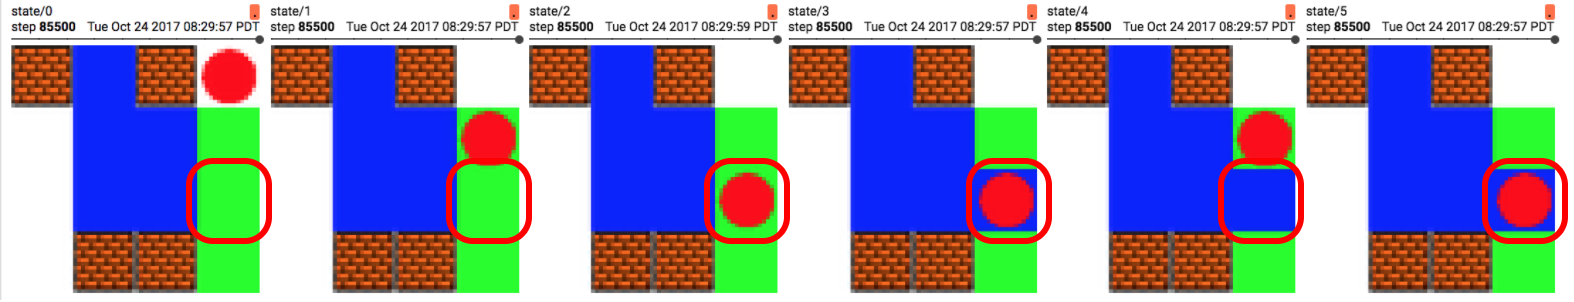
\includegraphics[width=.8\linewidth]{articles/icf/figures/ex1_env_5_step_boxed.png}}
\newline
\subfloat[]{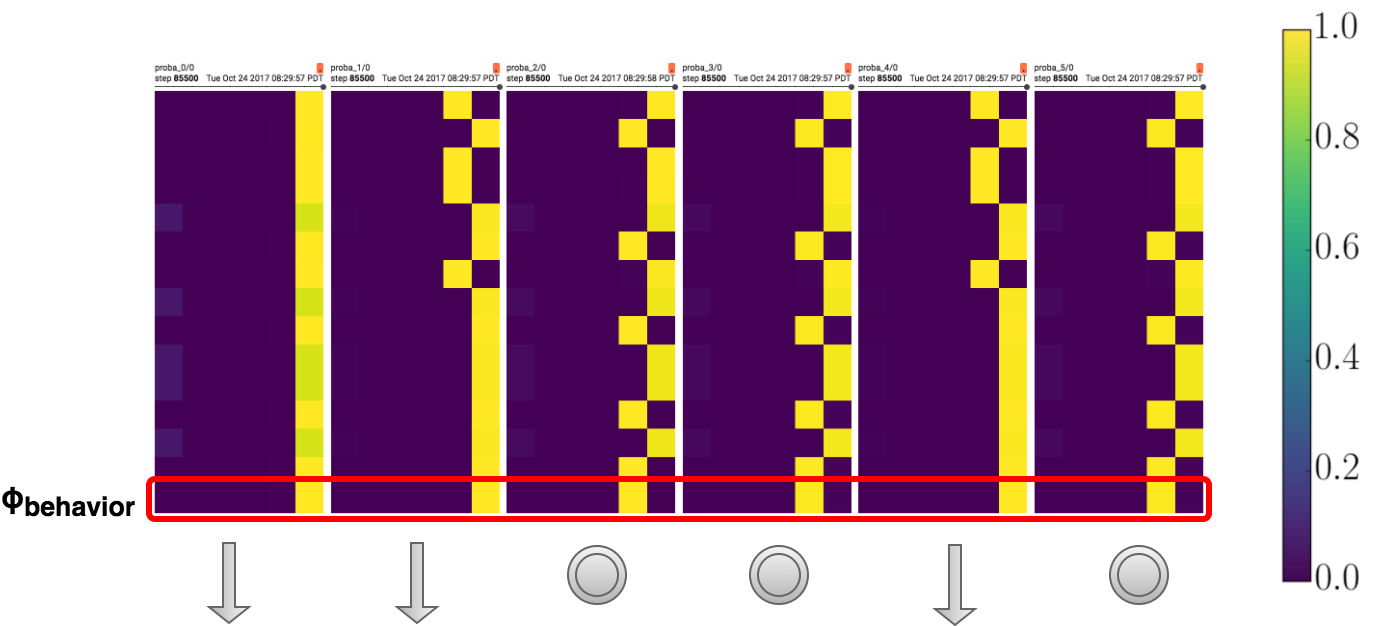
\includegraphics[width=.8\linewidth]{articles/icf/figures/ex1_action_probs_5_step_denoted_boxed.png}} 
\caption{(a) Mazebase environment over five time-steps.  Here the red dot denotes the position of the agent.  The $\phi_{behavior}$ governing the agent's policy appears to control toggling the switch indicated by the red rounded box. 
(b) Visualization of the policies instantiated by different $\phi$s.  Each box represents the probability distribution of the policies at that time step.  Each row is generated by a different $\phi$ and each column corresponds to an action (up, left, pass, right, toggle, down) in order.  The boxed column shows the $\phi_{behavior}$. The symbols below each box represent the most-probable action for the behavioral policy, where the grey circle indicates toggling the switch.}
\label{fig:multistep_toggle}
\end{figure}



\section{Variational bound and the selectivity}
\label{appendix:bound}
% \begin{tikzpicture}
\tikzstyle{main}=[circle, minimum size = 5mm, thick, draw =black!80, node distance = 7mm]
\tikzstyle{connect}=[-latex, thick]
\tikzstyle{box}=[rectangle, draw=black!100]
  \node[box,draw=white!100] (Latent) {\textbf{Latent}};
  \node[main] (a1) [right=of Latent] {$\va_1$};
  \node[main] (s1) [below=of a1] {$\vs_1$};
  \node[draw,thick, rounded corners, fit=(s1) (a1)] (L1) {};
  \node[main] (a2) [right=of a1] {$\va_2$};
  \node[main] (s2) [below=of a2] {$\vs_2$};
  \node[draw,thick, rounded corners, fit=(s2) (a2)] (L2) {};
  \node[main] (a3) [right=of a2] {$\va_3$};
  \node[main] (s3) [below=of a3] {$\vs_3$};
  \node[draw,thick, rounded corners, fit=(s3) (a3)] (L3) {};
  \node[main] (at) [right=of a3] {$\va_t$};
  \node[main] (st) [below=of at] {$\vs_t$};
  \node[draw,thick, rounded corners, fit=(st) (at)] (Lt) {};
  
  
  \node[box,draw=white!100] (Observed) [above=of Latent] {\textbf{Observed}};
  \node[main,fill=black!10] (O1) [right=of Observed,above=of L1] {$\gO_1$};
  \node[main,fill=black!10] (O2) [right=of O1,above=of L2] {$\gO_2$};
  \node[main,fill=black!10] (O3) [right=of O2,above=of L3] {$\gO_3$};
  \node[main,fill=black!10] (Ot) [right=of O3,above=of Lt] {$\gO_t$};

  \path (L3) -- node[auto=false]{\ldots} (Lt);
  \path (a1) edge [connect] (O1)
        (s1) edge [connect, bend right=45] (O1)
        (s1) edge [connect] (s2)
        (a1) edge [connect] (s2);
    \path (a2) edge [connect] (O2)
        (s2) edge [connect, bend right=45] (O2)
        (s2) edge [connect] (s3)
        (a2) edge [connect] (s3);
  \path (a3) edge [connect] (O3)
        (s3) edge [connect, bend right=45] (O3);
  \path (at) edge [connect] (Ot)
        (st) edge [connect, bend right=45] (Ot);
  \path (L3) -- node[auto=false]{\ldots} (Lt);

  \draw[dashed]  [below=of L1,above=of O1];
\end{tikzpicture}
Let us call $p(h_{t+1} | \phi_{t+1}, h_t) =  \mathcal{P}^\phi_{h' ,h}$ the probability distribution over final hidden states starting from $h$ and using the policy parametrized by the embedding $\phi$.

$p(h_{t+1} | \phi_{t+1}, h_t) = \Pi_{k=1}^{K}  \pi_{\phi_{t+1}}( a_{t+\frac{k-1}{K}} | h_{t+\frac{k-1}{K}}) p_{env}(s_{t+\frac{k}{K}} | a_{t+\frac{k-1}{K}}, s_{t+\frac{k-1}{K}})$.
where $p_{env}$ is the transition probability of the environment.
% $p(\bullet | \phi, h)$ 

For simplicity, let's refer to $h_t$ as $h$, $h_{t+1}$ as $h'$ and $\phi_{t+1}$ as $\phi$.
\subsection{Lower bound on the mutual information}
The bound $$\mathcal{I}_p(\phi, h' | h) \ge \sup_\theta  \mathbb{E}_{p(\phi|h)} \big[ \mathcal{S}(h, \phi)\big]$$ can be proven by using Donsker-Varadhan variational representation of the KL divergence \citep{donsker1975asymptotic,ruderman2012tighter}:

$$\kl{p}{q} = \sup_{T \in \mathcal{L}^\infty(q)} \mathbb{E}_p \big[ T  \big] - \log \mathbb{E}_q \big[ e^T \big]$$

For $A = e^T$ and using the identity $\mathcal{I}_p(X, Y) = \mathbb{E}_{p(y)} \big[ \kl{p(x|y)}{p(x)}\big]$ with $X=\phi|h$ and $Y=h'|h$, we have:

\begin{eqnarray*}
\mathcal{I}_p(\phi, h' | h) &=& \mathbb{E}_{h'|h} \sup_A \mathbb{E}_{\phi|h, h'} \big[ \log A(h', h, \phi) \big] - \log \mathbb{E}_{\varphi|h} \big[ A(h', h, \varphi) \big]\\
&=& \mathbb{E}_{h'|h} \sup_A \mathbb{E}_{\phi|h, h'} \big[ \log \frac{ A(h', h, \phi)}{\mathbb{E}_{\varphi|h} \big[ A(h', h, \varphi)\big]}\big]\\
&\ge&  \sup_A \mathbb{E}_{\phi|h}\mathbb{E}_{h'|\phi, h} \big[ \log \frac{ A(h', h, \phi)}{\mathbb{E}_{\varphi|h} \big[ A(h', h, \varphi)\big]}\big]\\
&\ge&  \sup_\theta \mathbb{E}_{\phi|h}\mathbb{E}_{h'|\phi, h} \big[ \log \frac{ A(h', h, \phi; \theta)}{\mathbb{E}_{\varphi|h} \big[ A(h', h, \varphi; \theta)\big]}\big]\\
\end{eqnarray*}
for parametric $A$ functions.

% In the case where $A(h', h, \phi)$ is actually is probability density $q(h' | h, \phi)$ (or any unnormalized density such that the normalization factor does not depend on $\phi$) we have:
% \begin{eqnarray*}
% \mathcal{S}(\phi, h) &=&\mathbb{E}_{h' \sim p
%     (h' | \phi, h)}  \log \frac{q(h' | \phi, h)}{\mathbb{E}_{\varphi | h} q(h' |
%     \varphi,
% h)}\\
% &=& \mathbb{E}_{\phi | h} \big[ {\kl{p(h'|\phi, h)}{q(h'|h)} -
% \kl{p(h'|\phi, h)}{q(h'|\phi, h)}} \big]\\
% &=& \mathbb{E}_{\phi | h} \big[ \kl{p(h'|\phi, h)}{q(h'|h)}\big] -
% \kl{p(h'| h)}{q(h'|h)} - \mathbb{E}_{p(h'|h)} \big[ \kl{p(\phi| h', h)}{q(\phi |h', h)}\big] \\
% &=& \mathbb{E}_{\phi | h} \big[ \kl{p(h'|\phi, h)}{p(h'|h)}\big]- \mathbb{E}_{p(h'|h)} \big[ \kl{p(\phi| h', h)}{q(\phi |h', h)}\big] \\
% &=& \mathcal{I}^{p} (\phi , h'|h) - \mathbb{E}_{p(h'|h)} \big[ \kl{p(\phi| h', h)}{q(\phi |h', h)}\big] \\
% % &=& \mathcal{I}^{p}(\phi \mapsto h')- \mathbb{E}_{p(h'|h)} \big[ \kl{p(\phi| h', h)}{q(\phi |h', h)}\big] \\
% \end{eqnarray*}
% where we used that fact that $p(\phi|h) = q(\phi|h)$ and by design we only sample $\phi$s from one generator.

% Thus, the gap between the selectivity and the mutual information is the KL divergence of the two posterior distributions.


As we sample the factors $\phi$ uniformly, our total objective is then a lower bound on $\sum_t \mathcal{I}(\phi_t, h_t | h_{t-1})$ which corresponds here to the \emph{directed information} \citep{massey1990causality} \cite{ziebart2010modeling} as $\phi_t$ is sampled independently from $\phi_{1:t-1}$.


% \input{equivariant_map.tex}


\section{Additional information on the training}

In our experiments, we use the selectivity objective, an autoencoding loss and an entropy regularization loss $\mathcal{H}(\pi_\phi)$ for each of the policies $\pi_\phi$. Furthermore, in experiment 4.2 we added the model-based cost $||h' - T(h, \phi)||^2$ with $T$ a learned two layer fully connected neural network.

The selectivity is used to update the parameters of the encoder, factor generator and policy networks.
We use the following equation for computing the gradients

$$\nabla_\theta \mathbb{E}_{\pi_\theta} \big[ f_\theta \big] =  \mathbb{E}_{\pi_\theta} \big[ \nabla_\theta f_\theta + f_\theta \nabla_\theta \log \pi_\theta \big]$$ 
We also use a state dependent baseline $V$ as a control variate to reduce the variance of the REINFORCE estimator.

Furthermore, to be able to train the factor generator efficiently, we train all $\phi$ sampled in a mini-batch (of size $1024$) by importance sampling on the probability ratio of the trajectory under each $\phi$
